%% Example of a LaTeX source file for a COLING-2012 submission
%% last updated: July 10, 2012
%% Optional instructions for authors within the tex file are provided as comments and start with 'for authors:...'
\documentclass[10pt,a5paper,twoside]{article}
\usepackage{coling2012}
\usepackage{comment}
\usepackage{amsmath}
%\title{Translating to Shakespeare: A Case Study in Paraphrasing Writing Styles}
\title{You can be Shakespeare! \\ A Case Study in Paraphrase Targeting Writing Styles}
%for authors: in case of more than four author names ref. to commented line below 
%\author{$Annie~SMITH^{1, 2}~~~LI~Xiao Dong^{1, 3}$\\$~~~Third~Author^{1, 2}~~~Fourth~Author^{1, 3}~~~ Fifth~Author^{2, 3}$\\
\author{$Author1^{1, 2}~~~Author2^{1, 3}$\\
{\small  	(1) INSTITUTE\_1, address 1\\ 
 		(2) INSTITUTE\_2, address 2\\
		(3) INSTITUTE\_3, address 3\\
  \texttt{author1@institute1, author@institute2} \\ 
}}

\begin{document}
\maketitle
%% The first mandatory ABSTRACT (\abstractEn) section below is for the English language
\abstractEn{  %ABSTRACT}{
We present initial investigation into the task of paraphrasing language while targeting a particular writing style.
The plays of William Shakespeare and their modern translations are used as a testbed for evaluating
paraphrase systems targeting a specific style of writing.
%We demonstrate that existing evaluation metrics developed in the Machine Translation and Paraphrase communities are
%insufficient when the goal is to generate paraphrases targeting a specific style, and
%propose a series of new metrics to measure how closely the generated paraphrases match the target
%style.  
We show that even with a relatively small amount of parallel training data available, it is
possible to learn paraphrase models which capture stylistic phenomenon, and these models outperform
baselines based on dictionaries and out-of-domain parallel text.
In addition we present an initial investigation into automatic evaluation metrics for paraphrasing writing style.
To the best of our knowledge this is the first work to investigate the task of
paraphrasing text with the goal of targeting a specific style of writing.
}

\keywordsEn{Paraphrase, Writing Style}

\section{Introduction}
%The plays of William Shakespeare and their \emph{modern} translations are treated
%as parallel text which is used to learn paraphrase models targeting the style of Early Modern English employed by Shakespeare.

Identical meaning can be expressed or \emph{paraphrased} in many different ways; automatically detecting or generating different expressions with the same meaning is 
fundamental to many natural language understanding tasks\cite{Giampiccolo07}, so much previous work has investigated methods for automatic paraphrasing\cite{Barzilay03,dolan04,Shinyama03,Das09,bannard05}.  

Although two utternaces might be semantically equivelant, they can still be stylistically quite different.  For example, the same information
is likely to be conveyed using very different lexical and grammatical patterns in advertising materials v.s. technical manuals, or in Shakespearean plays v.s. Hollywood movies.

Systems capable of paraphrasing text targeting to a specific writing style could be useful for a variety of applications.  For example, they could:
\begin{enumerate}
  \item Help authors of technical documents to adhere to appropriate stylistic guidelines.  
  \item Enable average people to better understand information in legal documents by translating ``leaglese'' into ordinary English.  
  \item Benefit educational applications:
    \begin{enumerate}
    \item Students studying a specific style of writing may benefit from access to \emph{modern english} versions of works by authors they are studying.
    \item Automatic paraphrases could help students to experiment with writing in the style of the authors whose works they are reading.
    \end{enumerate}
\end{enumerate}

In this paper, we investigate the task of automatic paraphrasing when targeting a writing style, focusing specifically on the style of Early Modern English employed by William Shakespeare.
We exploit modern translations of 17 plays written to help students better understand Shakespeare's work.  A parallel corpus is extracted from these modern translations,
which is then used to train phrase-based translation models which are capable of automatically paraphrasing ordinary sentences into Shakesperean English.  In addition we develop several
baseline systems which do not make use of this source of parallel text and instead rely on manually compiled dictionaries of expressions commonly found in Shakesperean english, or out of
domain parallel monolingual text gathered through Amazon's Mechanical Turk \cite{chen11}.

We evaluate these models both through human judgements and standard evaluation metrics from the Machine Translation and paraphrase literature, however no previous work has investigated the ability of automatic
evaluation metrics to capture the notion of writing style.  
We show that previously proposed automatic evaluation metrics do not give us a complete picture of a system's performance when the task is to generate paraphrases
targeting a specific style of writing.  We propose several new metrics for evaluating paraphrases targeting a specific style, and measure correlation with human judgements showing promising
preliminary results.

Systems which are capable of automatically paraphrasing literary writing styles could be directly benefical for educational applications.  For example, our systems which generate paraphrases targeting
a Shakesperean English could help students to experiment with writing literature in this style.
In addition, out of the 37 surviving plays written by William Shakespeare modern translations are currently only available for 17.  Though we have not yet formally evaluated
paraphrasing Shakespeare's plays into modern English, we believe it should be possible to help make the other 20 plays more accessable to students of Shakespeare by automatically 
generating modern translations.

\section{Shakesperean Paraphrasing}
We propose to use Shakespeare's plays as a testbed for the task of paraphrasing while targeting a specific writing style.  Because these plays are some of the
highest regarded examples of English literature and are also very unique in style, many linguistic resources are available such as parallel corpora
of modern translations and dictionaries of stylistically representative words and their modern equivelants.

We compare 3 different stylisitic paraphrase systems targeting Shakesperean English.  One which leverages parallel corpora of modern translations, another which makes use
of dictionaries of styalistically representative expressions, and another which leverages out-of-domain monolingual parallel data.

\subsection{Modern Translations}
Having access to parallel text in the target style allows us to train statistical models for generating paraphrases, and also perform automatic evaluation of semantic adequacy using BLEU, which requires access to a set of reference translations.  For this purpose we scraped modern translations of 17 Shakespeare plays from \url{http://nfs.sparknotes.com}, and an additional 8 translations of overlapping plays from \url{http://enotes.com}, giving us two reference translations for 8 out of the 17 plays.

After tokenizing and lowercasing, the plays were aligned using Bob Moore's bilingual sentence aligner \cite{Moore02}, which produced about 21,079 alignments out of 31,718 sentences in the Sparknotes data, and 10,365 sentence pairs out of 13,640 sentences in the enotes data.  The modern translations from each source are qualitatively quite
different.  The Sparknotes paraphrases tend to differ significantly from the original text, whereas the enotes translations are much more conservative, making fewer changes.
To illustrate these differences empirically and provide an initial paraphrase baseline, we computed BLEU scores of the unchanged modern translations against Shakespeare's 
original text; the Sparknotes paraphrases result in a BLEU score of 24.67, whereas the Enotes paraphrases prouce a much higher BLEU of 52.30 indicating their strong similarity to the original plays.
These corpus statistics are summarized in table \ref{corpus_stats}.

\begin{table}
  \begin{center}
    \begin{tabular}{|l|r|r|r|}
      \hline
      corpus & initial size & aligned size & No-Change BLEU\\
      \hline
      \hline
      \url{http://nfs.sparknotes.com} & 31,718 & 21,079 & 24.67 \\
      \hline
      \url{http://enotes.com} & 13,640 & 10,365 & 52.30 \\
      \hline
    \end{tabular}
  \end{center}
  \caption{Parallel corpora generated form modern translations of Shakespeare's plays}
  \label{corpus_stats}
\end{table}

To generate paraphrases, we apply a typical phrase-based Statistical Machine Translation pipeline, performing
word alignment on the data described in table \ref{corpus_stats} using GIZA++ \cite{Och03}, then extracting phrase pairs and performing decoding using Moses \cite{Koehn07}.

\subsection{Baselines}
Phrase-based translation has been demonstrated to be an effective approach to generating paraphrses \cite{chen11,quirk04}, however this approach does require the existence of
parallel corpora which may not be available for many writing styles.  For this reason we were motivated to investigate alternative approaches.

\subsubsection{Dictionary Based Paraphrase}
\label{dictionary_baseline}
Several dictionaries of stylistically representative words of Shakesperean English and their modern equivelants are available on the web.  These dictionaries can be used 
to define a translation model which is used in combination with a language model as in standard phrase-based MT \cite{Koehn00}.

%We gathered a set of 20,138 dictionary entries which were scraped from \url{http://www.shakespeareswords.com/}, then used heuristic rules to extract 68,709 phrase/word pairs.  Example
%dictionary entries are presented in table \ref{dictionary_example}. As described in \cite{Koehn00}, we estimate phrase translation probabilities based on the frequencies of the translation words/phrases in the target language - the Shakespearean English. 

We scraped a set of 68,709 phrase/word pairs from \url{http://www.shakespeareswords.com/}.  
Example dictionary entries are presented in table \ref{dictionary_example}. 

%As described in \cite{Koehn00}, we estimate phrase translation probabilities based on the frequencies of the translation words/phrases in the target language - the Shakespearean English. 
As described in \cite{Koehn00}, we estimate phrase translation probabilities based on the frequencies of the translation words/phrases in the target language (Shakespearean English).
For instance, if we look at the modern English word \emph{maybe}, our dictionary lists 4 possible Shakespearean translations. 
We obtained the conditional probabilities for each translation according to the n-gram back off model built on Shakespeare's 
36 plays by SRILM toolkit \cite{Stolcke02} \ref{word_frequency}, 
normalizing the probabilities for each source phrase, for example $p(\text{PERCHANGE}|\text{maybe}) = \frac{0.0000790755}{0.00026264791} = 0.30107035689$. 
This method allows us to estimate reasonable translation probabilities for use in a phrase table, which is used in combination 
with a language model consisting of Shakespeare's 36 plays (holding out Romeo and Juliet), which are then fed into the Moses decoder
\cite{Koehn07}.

\begin{table}
  \begin{center}
  \begin{tabular}{|l|l||l|l|}
    \hline
    target & source & target & source \\
    \hline
    \hline
    ABATE & shorten & AYE & always \\
    \hline
    CAUTEL & deceit & GLASS & mirror \\
    \hline
    SUP & have supper & VOICE & vote \\
    \hline
  \end{tabular}
  \end{center}
  \caption{Exaple dictionary entries}
  \label{dictionary_example}
\end{table}

\begin{table}
  \begin{center}
  \begin{tabular}{|l|l|l|}
    \hline
    Smoothed Probability Estimate & target & source \\
    \hline
    \hline
    0.0000790755 & PERCHANCE & maybe \\
    \hline
    0.00003691883 & PERADVENTURE & maybe \\
    \hline
    0.00007524298 & HAPLY & maybe \\
    \hline
    0.00007141065 & HAPPILY & maybe \\
    \hline
    \hline
    total 0.00026264791 & & \\
    \hline
  \end{tabular}
  \end{center}
  \caption{Example ngram probabilities in target language}
  \label{word_frequency}
\end{table}

\subsubsection{Out of Domain Monolingual Parallel Data}
As a final baseline we consider a paraphrase system which is trained on out-of-domain data gathered by asking users of Amazon's Mechanical Turk Service 
\cite{Snow08} to describe videos \cite{chen11}.  We combine a phrase table extracted from this out of doimain parallel text, with an in-domain
language model consisting of Shakespeare's 36 plays (holding out Romeo and Juliet for testing), applying the Moses decoder \cite{Koehn07} to find the best paraphrases. 
Although this monolingual parallel data does not include text in the target writing style,
the in-domain language model does bias the system's output towards Shakespeare's style of writing.

\subsection{Comparison Using Existing Automatic Evaluation Metrics}
Figure \ref{bleupinc} compares a variety of sytstems targeting Shakesperean English using the previosly proposed BLEU \cite{Papineni02} and PINC \cite{chen11} automatic evaluation metrics which
have been demonstrated to correlate with human judgements on semantic adequacy and lexical dissimilarity with the input.
A description of each of the systems compared in this experiment is presented in table \ref{systems}.  Notice that the Enotes paraphrases are quite similar to the original text,
obtaining a BLEU score of 52.3 when compared directly to the original lines from Shakespeare's plays.  Because our goal is to produce paraphrases which make more dramatic stylistic changes to the input,
in the remainder of this paper, we focus on the Sparknotes data for evaluation.

\subsubsection{Discussion}
Two main trends emerge from Figure \ref{bleupinc}.  First, notice that all of the systems which are trained using parallel text achieve higher BLEU scores than the baseline
of not making any changes to the modern translations.  While the dictionary baseline achieves a competitive PINC score, indicating it is making a significant number of changes to the 
input, it's BLEU is lower than the \emph{no changes} baseline.  Secondly, it seems apparent that the systems whose parameters are learned using Minimum Error Rate Training \cite{MERT}
tend to be more conservative, making fewer changes to the input and thus achieving lower PINC scores, however also not seeing any BLEU improvements on the test data.  Finally
we note that using the larger language model seems to yield a slight improvement in BLEU score.

\subsection{Examples}
Several example paraphrases of lines from Romeo and Juliet and a few Hollywood movies, generated by the top performing system according to BLEU and PINC, are presented in table \ref{examples}.

\begin{table}[ht]
  \begin{center}
    \begin{tabular}{|l|p{3in}|}
      \hline
      System & Description \\
      \hline
      \hline
      16and7plays\_36LM & Phrase table learned from all 16 Sparknotes plays (other than R\&J) and language model built from all 36 of Shakespeare's plays, excluding R\&J.
      Uses default Moses parameters. \\
      \hline
      16and7plays\_36LM\_MERT & Same as 16and7plays\_36LM except parameters are tuned using Minimum Error Rate Training \cite{MERT} instead of using the default Moses parameters.\\
      \hline
      16and7plays\_16LM & Phrase table is built from both Sparknotes and Enotes data, and Language model is built from the 16 with modern translations\\
      \hline
      16and7plays\_16LM\_MERT & Same as 16and7plays\_16LM except parameters are tuned using MERT. \\
      \hline
      16plays\_36LM & Only Sparknotes modern translations are used.  All 36 plays are used to train Shakesperean language model. a\\
      \hline
      16plays\_36LM\_MERT & Same as 16plays\_36LM except parameters are tuned using MERT. \\
      \hline
      modern (no change) & No changes are made to the input, modern translations are left unchanged. \\
      \hline
      Dictionary & Dictionary baseline described in section \ref{dictionary_baseline}\\
      \hline
    \end{tabular}
  \end{center}
  \caption{Descriptions of various systems for Shakesperean Paraphrase.  Romeo and Juliet is held out for testing.}
  \label{systems}
\end{table}

\begin{figure}
  \begin{center}
    \begin{tabular}{cc}
      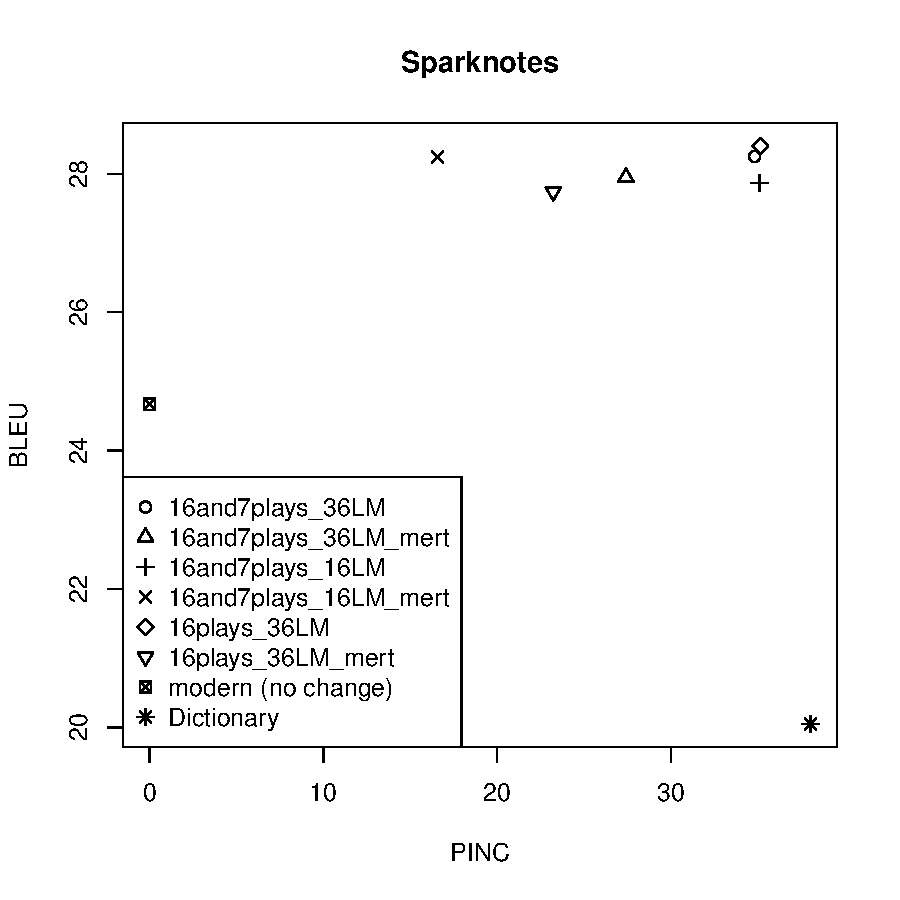
\includegraphics[width=2.4in]{figures/bleupinc1.pdf} & 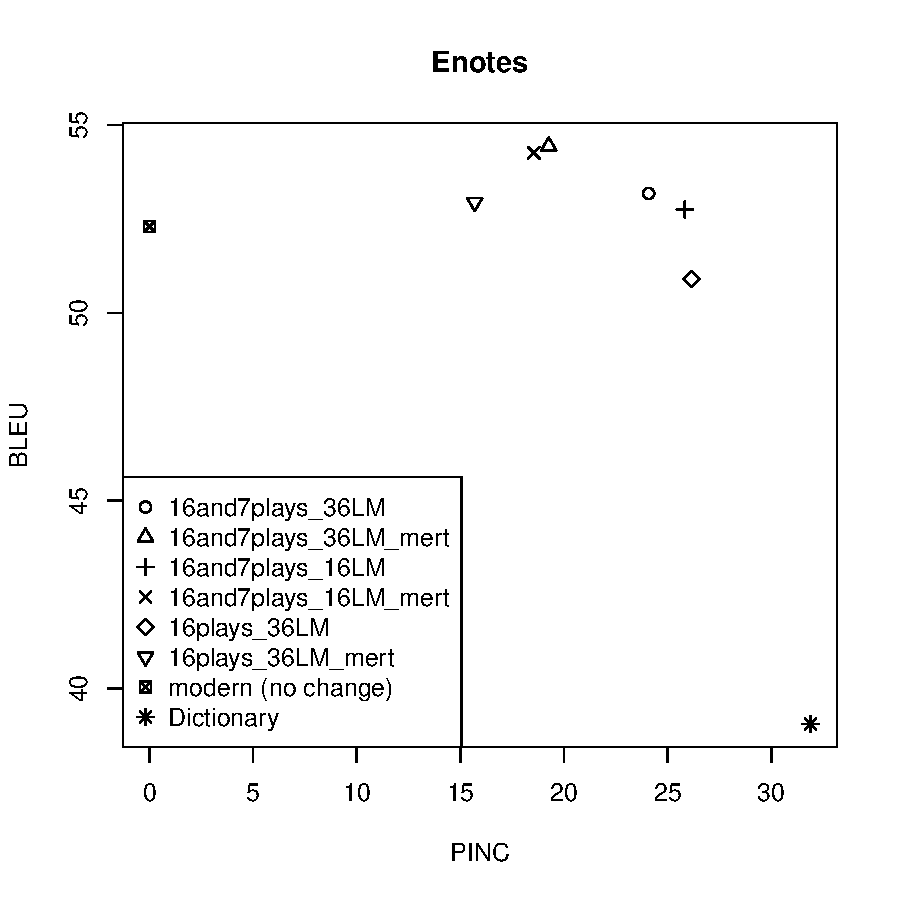
\includegraphics[width=2.4in]{figures/bleupinc2.pdf} \\
    \end{tabular}
  \end{center}
  \caption{Various Shakesperean Paraphrase systems compared using BLEU and PINC.  A brief description of each system is presented in table \ref{systems}.}
  \label{bleupinc}
\end{figure}

\begin{table}[ht]
  \begin{center}
    \begin{tabular}{|l|l|p{1.4in}|p{1.4in}|}
      \hline
      Source & Speaker & Input & Output \\
      \hline
      \hline
      Romeo \& Juliet & Benvolio & he killed your relative , brave mercutio , and then young romeo killed him . & he slew thy kinsman , brave mercutio , and then young romeo kill him . \\
      \hline
      Romeo \& Juliet & Romeo & i can read my own fortune in my misery . & i can read mine own fortune in my woes . \\
      \hline
      Star Wars & Palpatine & If you will not be turned, you will be destroyed! & if you will not be turn 'd , you will be undone ! \\
      \hline
      Star Wars & Luke & Father, please! Help me! & father , i pray you , help me ! \\    
      \hline
      The Matrix & Agent Smith & Good bye, Mr. Anderson. & fare you well , good master anderson . \\
      \hline
      The Matrix & Morpheus & I'm trying to free your mind, Neo. But I can only show you the door. You're the one that has to walk through it. & i 'll to free your mind , neo. but i can but show you the door. you 're the one that hath to tread it . \\
      \hline
      Raiders of the Lost Ark & Belloq & Good afternoon, Dr. Jones. & well met , dr. jones . \\
      \hline
      Raiders of the Lost Ark & Jones & I ought to kill you right now. & i should kill thee straight . \\
      \hline
    \end{tabular}
  \end{center}
  \caption{Example Shakesperean paraphrases generated by the best overall system.}
  \label{examples}
\end{table}

\section{Human Evaluation}
\label{human_evaluation}
Figure \ref{bleupinc} provides some insight into the performance of the various systems, however it is innitially unclear how well the BLEU and PINC
automatic evaluation metrics perform when applied to evaluating paraphrases targeting a specific style of writing.  BLEU and PINC have previously
been shown to have high correlation with human judgements of semantic adequacy and lexical dissimilarity of paraphrase candidates, however no
previous work has evaluated automatically generated paraphrases which target a specific style of writing \cite{chen11}.

While BLEU is typically used to measure semantic adequacy, it seems reasonable to assume that it may also depend on style, since utterances
are more likely to contain overlapping ngrams if they are both semantically and stylistically similar.  What BLEU doesn't tell us, however
is what portion of it's improvements are due to stylistic similarity or semantic equivelance.  For this reason, we were motivated perform
an evaluation based on human judgements of semantic adequacy, lexical dissimilarity and stylistic similarity.

For this purpose, we randomly sampled 100 lines from Romeo and Juliet, then two of the authors annotated each sentence and it's Shakesperean
translation with semantic adequacy, lexical dissimilarity, stylistic similarity, and overal quality.
The aggregate results of the human evaluation are displayed in figure \ref{human_judgements}.  Agreement between annotators
measured using Pearson's $\rho$ is displayed in table \ref{annotator_agreement}.

Based on the human evaluation, it appears that the baseline combining paraphrases collected from mechanical turk \cite{chen11} with
a Shakesperean language model has the highest semantic adequacy, however it is also fairly conservative making few changes to the input.

The dictionary baseline, and paraphrase system trained on parallel modern translations are roughly comparable when it comes to 
the number of changes made to the input, however the system trained on modern translations achieves higher semantic adequacy, while also being rated higher on style and overall.

These results are roughly in line with the automatic evalution metrics presented in figure \ref{bleupinc}, however we see several important
trends which are not aparent based on the automatic evaluation metrics.

Although the video baseline achieves the highest semantic adequacy in the human evaluation, it's BLEU score
is significantly lower than 16plays\_36LM on the Sparknotes data.\footnote{
Note that the BLEU score of 16plays\_36LM is significantly lower when evaluated on the Enotes data.  This makes sense, because the 
16 plays come from Sparknotes. This system is not trained on the 7 Enotes plays which, whose modern translations tend
to be slightly different in style.}
It would appear that in this case BLEU is conflating semantic adequecy with writing style.  Although the paraphrases produced 
by the video baseline have high semantic adequacy, their style tends to differ substantially from the reference translations resulting
in fewer ngram matches, and thus a lower BLEU score.

\begin{table}[ht]
  \begin{center}
    \begin{tabular}{|l|l|l|l|}
      \hline
      Semantic Adequacy & Lexical Dissimilarity & Style & Overall \\
      \hline
      \hline
      0.73 & 0.82 & 0.64 & 0.62 \\
      \hline
    \end{tabular}
  \end{center}
  \caption{Agreement between annotators measured using Pearson's $\rho$.}
  \label{annotator_agreement}
\end{table}

\begin{figure}
  \begin{center}
    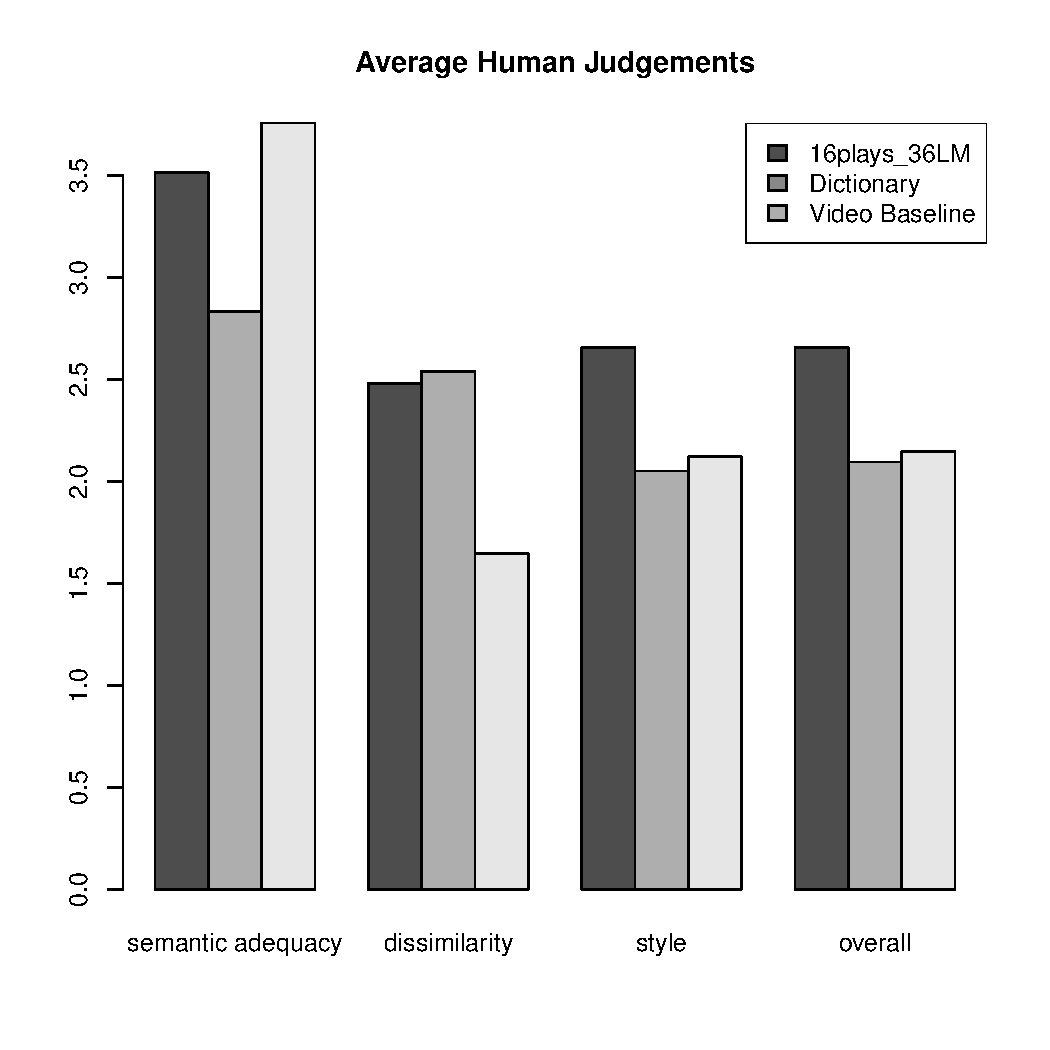
\includegraphics[width=5in]{figures/human_judgements.pdf}
  \end{center}
  \caption{Average human judgements evaluating semantic adequacy, lexical dissimilarity, stylistic similarity, and overall quality
    of Shakesperean paraphrase systems} 
  \label{human_judgements}
\end{figure}

\section{Automatic Metrics Evaluating Writing Style}
While PINC and BLEU do seem useful for automatically evaluating paraphrases targeting a  writing style, BLEU tends to conflate the notions of
semantic adequacy with writing style.  When comparing various systems using automatic metrics, it would seem useful
to seperate effects based on these two critera.  We would like our automatic evaluation metrics to be able to distinguish
between a system which generates perfect paraphrases which don't match the target style of writing and a system which
generates sentences in the correct style, but which convey different meaning.

To help address this issue we propse two new automatic evaluation metrics whose goal is to measure the degree to which
autoamtic paraphrases match the target style.  Both metrics assume existence of large corpora in both the source and
target style, but do not require access to any parallel text, or human judgements.

We present a preliminary evalutation of these metrics by measuring their correlation with human judgements, however
we emphasize that we are only evaluating these metrics with respect to one specific style of writing.  We
are cautionsly optimistic that our results will generalize across writing styles, however, as they are based entirely
on ngram statistics.

\subsection{Cosine Similarity Style Metric}
As a first approach automatic evaluation of writing style, we propose a vector-space model of similarity between the system
output and a large corpus of text in both the source and target style.  The intuition is that if there is a large ngram
overlap between the system's output and a large corpus of text in the target style, then the output is more likely to be
stylistically appropriate.

More concretely, we extract ngrams from both the source and target corpus which are then represented as binary
vectors $\vec{s}$, and $\vec{t}$; similarly the output sentence is represented using a vector of
ngrams $\vec{o}$.  
The proposed metric is the normalized cosine similarity between the source and target corpora:
\[
S_{\text{Cosine}}(\vec{o}) = \frac{\frac{\vec{o} \cdot \vec{t}}{\|\vec{o}\| \times \|\vec{t}\|}}{\frac{\vec{o} \cdot \vec{t}}{\|\vec{o}\| \times \|\vec{t}\|} + \frac{\vec{o} \cdot \vec{s}}{\|\vec{o}\| \times \|\vec{s}\|}}
\]
 

\subsection{Logistic Regression Style Metric}
We also consider a Logistic Regression based approach as an alternative to the Cosine-Similarity based style metric.  Here the idea is to estimate the probability that each
sentence belongs to the target style based on the ngrams it contains, using large corpora of in and out-of domain sentences to learn  parameters of a logistic regression model.

The probability a sentence belongs to the target style is estimated as follows:
\[
%P(\text{style} = \text{target}|\text{output}) \propto \text{exp} \left( \vec{\theta} \cdot \vec{f(\text{output})} \right)
P(\text{style} = \text{target}|\text{sentence}) = \frac{1}{1 + e^{-\left( \vec{\theta} \cdot \vec{f(\text{sentence})} \right)}}
\]
Where $\vec{f(\text{sentence})}$ is a vector of ngrams, and $\vec{\theta}$ is a vector of weights.  

The parameters, $\vec{\theta}$, are optimized on the source and target corpus, where the assumption is that the target corpus
is in the target style, whereas the source corpus is not.\footnote{
  Parameters were optimized using MEGAM \url{http://www.cs.utah.edu/~hal/megam/}.
}

\subsection{Evaluation}
We trained both Logistic Regression and Cosine Similarity evaluation metrics using the original Shakespeare plays and modern translations as
the source and target corpus respectively (holding out Romeo and Juliet), then measured Pearson's Correlation Coefficent between the automatic
evaluation metrics and human judgements reported in section \ref{human_evaluation}.  These results are reported in table \ref{correlation}.

\begin{table}
  \begin{center}
  \begin{tabular}{|l|l|r|}
    \hline
    & & Pearson's $\rho$ \\
    \hline
    \hline
    semantic adequacy & BLEU & 0.35 \\
    \hline
    dissimilarity & PINC & 0.78 \\
    \hline
    style & BLEU & 0.07 \\
    \hline
    style & PINC & 0.20 \\
    \hline
    style & Cosine & 0.37 \\
    \hline
    style & Maximum Entropy & 0.47 \\
    \hline
  \end{tabular}
  \end{center}
  \caption{Correlation between various human judgements and automatic evaluation metrics}
  \label{correlation}
\end{table}

As can be seen in table \ref{correlation}, the correlation between semantic adequacy and BLEU appears smaller than that reported in previous work \cite{chen11}.  Presumably this is
due to the conflation of stylistic differences and semantic adequacy discussed discussed in section \ref{human_evaluation}, however it also appears 
that the correlation between BLEU and human style judgements is too low to be of practical use for evaluating style.

PINC, on the other hand has high correlation with judgments on dissimilarity, and is also moderately correlated with human style
judgements.  We believe PINC has some correlation with writing style, because the systems we are evaluating all target Shakesperean English, 
so whenever changes are made to the input, they are likely to make it similar to the target style.
Although PINC has relatively high correlation with human judgements, it is likely not a very useful measure of writing style in practice.
For example, consider a paraphrase system which makes many changes to the input and thus gets a high PINC score, but targets a completely different writing style.

Both the Cosine and Maximum Entropy style metrics achieve the highest overall correlation with human writing style judgements, with the Maximum Entropy style score performing significantly better.

Finally we note that overall the automatc metrics tend to agree with agree with human judgements as displayed in figure \ref{style_metrics}.

\begin{figure}
  \begin{center}
    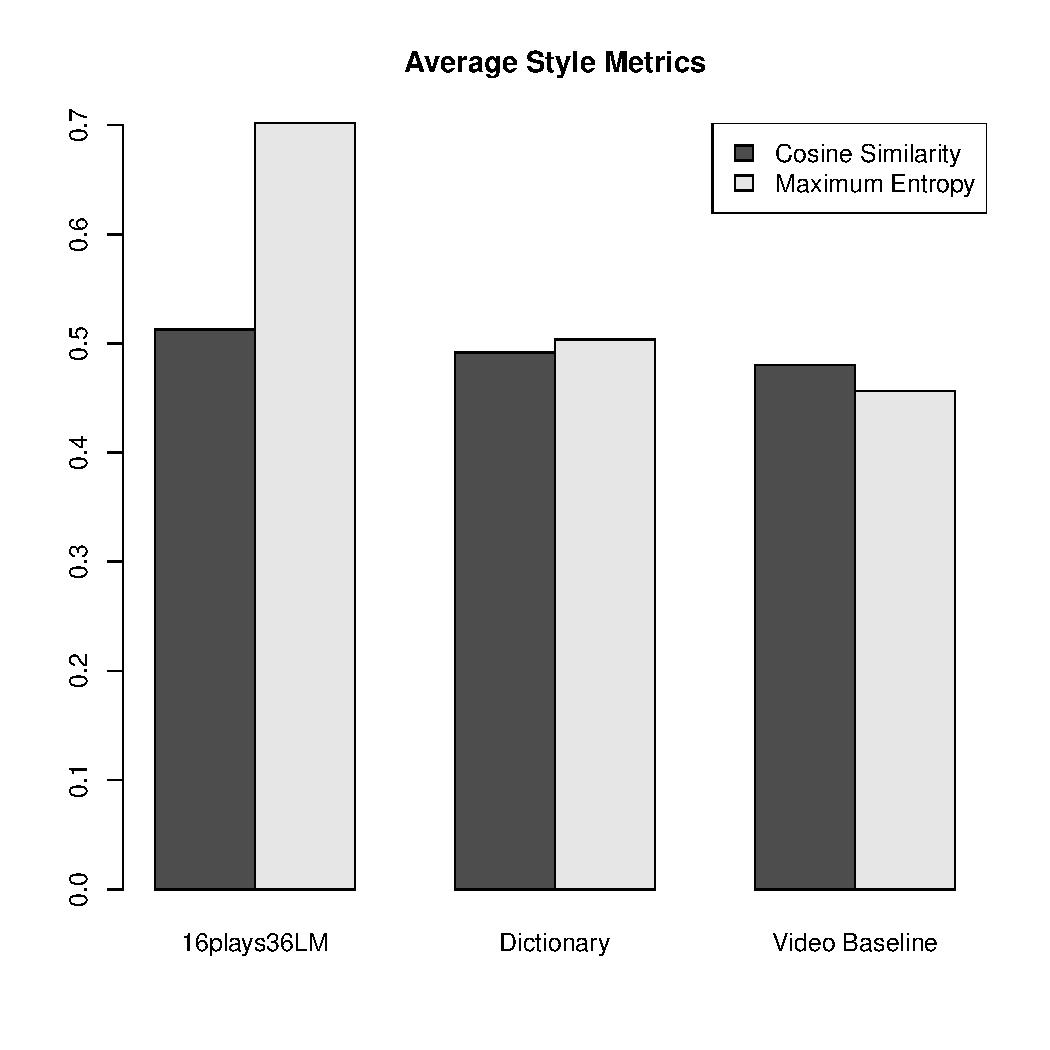
\includegraphics[width=5in]{figures/style_metrics.pdf}
    \end{center}
    \caption{Overall results from comparing automatic style metrics.  Note that the automatic metrics agree with results from human judgements in figure \ref{human_judgements}.}
    \label{style_metrics}
\end{figure}

\section{Related Work}
Although no previous work has investigated paraphrasing modern text into Shakesperean English, or the more general task of paraphrasing while targeting a specific writing
style, we highlight several strands of related work.

Perhaps most relevant is recent work generating and translating rhythmic poetry \cite{Greene10}.  This work focuses on automatically generating text in an appropriate
meter (e.g. iambic pentameter) using finate-state transducers, however doesn't address the issue of paraphrase.  
While our work does not address the issue of meter, it should be possible to combine our translation
models with their weighted Finate State Transducers to produce Shakesperean paraphrase models which produce output in an appropriate meter.

Much previous work has addressed the task of automatically generating paraphrases \cite{Barzilay03,dolan04,Shinyama03,Das09,bannard05,Callison-Burch08,Kok10}.  In addition several authors have previously proposed 
automatic paraphrase evaluation metrics \cite{chen11,Callison-Burch08b,Bangalore00,liu10} for paraphrase.
We are not aware, however, of any previous work that has addressed the task of generating or evaluating
paraphrases targeting a specific style of writing.

Finally we highlight related work on authorship classification which can be seen as detecting a specific style of writing \cite{Gamon04,Raghavan10}.
This work has not specifically addressed the task of automatically generating or evaluating paraphrases in a specific style.

\section{Conclusions}
We have presented initial investigation into the task of automatic paraphrasing while targeting a specific style of writing.  We proposed Shakespere's plays and their
modern translations as a tesbed for this task, and developed a series of paraphrase systems targeting Shakesperean English.  We showed that while existing evaluation
metrics are useful for evaluating paraphrases in this context, BLEU tends to conflate semantic equivelance with writing style giving an incomplete picture of which systems
perform better according to each of these critera.  

To address the problems we have demonstrated with previous evaluation metrics applied to this task, we have introduced two new metrics for evaluating writing style.
We measured correlation between automatic metrics and human judgements in the context of paraphrasing writing style, and showed
that our new metrics have better correlation with human judgements than existing metrics in the context of our data.
While this evaluation is limited to one specific style of writing, we are optimistic that these or similar metrics will also perform well when
evaluating other writing styles.

Future work could include automatically translating the remaining 20 of Shakespeare's plays into modern English, which could be benefical to students
of Shakespere's plays and also to future human translators.

\bibliographystyle{apa}

\bibliography{paper.bib}

%%================================================================
\end{document}
